\documentclass[man]{apa6}

\usepackage{amssymb,amsmath}
\usepackage{ifxetex,ifluatex}
\usepackage{fixltx2e} % provides \textsubscript
\ifnum 0\ifxetex 1\fi\ifluatex 1\fi=0 % if pdftex
  \usepackage[T1]{fontenc}
  \usepackage[utf8]{inputenc}
\else % if luatex or xelatex
  \ifxetex
    \usepackage{mathspec}
    \usepackage{xltxtra,xunicode}
  \else
    \usepackage{fontspec}
  \fi
  \defaultfontfeatures{Mapping=tex-text,Scale=MatchLowercase}
  \newcommand{\euro}{€}
\fi
% use upquote if available, for straight quotes in verbatim environments
\IfFileExists{upquote.sty}{\usepackage{upquote}}{}
% use microtype if available
\IfFileExists{microtype.sty}{\usepackage{microtype}}{}

% Table formatting
\usepackage{longtable, booktabs}
\usepackage{lscape}
% \usepackage[counterclockwise]{rotating}   % Landscape page setup for large tables
\usepackage{multirow}		% Table styling
\usepackage{tabularx}		% Control Column width
\usepackage[flushleft]{threeparttable}	% Allows for three part tables with a specified notes section
\usepackage{threeparttablex}            % Lets threeparttable work with longtable

% Create new environments so endfloat can handle them
% \newenvironment{ltable}
%   {\begin{landscape}\begin{center}\begin{threeparttable}}
%   {\end{threeparttable}\end{center}\end{landscape}}

\newenvironment{lltable}
  {\begin{landscape}\begin{center}\begin{ThreePartTable}}
  {\end{ThreePartTable}\end{center}\end{landscape}}

  \usepackage{ifthen} % Only add declarations when endfloat package is loaded
  \ifthenelse{\equal{\string man}{\string man}}{%
   \DeclareDelayedFloatFlavor{ThreePartTable}{table} % Make endfloat play with longtable
   % \DeclareDelayedFloatFlavor{ltable}{table} % Make endfloat play with lscape
   \DeclareDelayedFloatFlavor{lltable}{table} % Make endfloat play with lscape & longtable
  }{}%



% The following enables adjusting longtable caption width to table width
% Solution found at http://golatex.de/longtable-mit-caption-so-breit-wie-die-tabelle-t15767.html
\makeatletter
\newcommand\LastLTentrywidth{1em}
\newlength\longtablewidth
\setlength{\longtablewidth}{1in}
\newcommand\getlongtablewidth{%
 \begingroup
  \ifcsname LT@\roman{LT@tables}\endcsname
  \global\longtablewidth=0pt
  \renewcommand\LT@entry[2]{\global\advance\longtablewidth by ##2\relax\gdef\LastLTentrywidth{##2}}%
  \@nameuse{LT@\roman{LT@tables}}%
  \fi
\endgroup}


  \usepackage{graphicx}
  \makeatletter
  \def\maxwidth{\ifdim\Gin@nat@width>\linewidth\linewidth\else\Gin@nat@width\fi}
  \def\maxheight{\ifdim\Gin@nat@height>\textheight\textheight\else\Gin@nat@height\fi}
  \makeatother
  % Scale images if necessary, so that they will not overflow the page
  % margins by default, and it is still possible to overwrite the defaults
  % using explicit options in \includegraphics[width, height, ...]{}
  \setkeys{Gin}{width=\maxwidth,height=\maxheight,keepaspectratio}
\ifxetex
  \usepackage[setpagesize=false, % page size defined by xetex
              unicode=false, % unicode breaks when used with xetex
              xetex]{hyperref}
\else
  \usepackage[unicode=true]{hyperref}
\fi
\hypersetup{breaklinks=true,
            pdfauthor={},
            pdftitle={Assignment Statistics 6},
            colorlinks=true,
            citecolor=blue,
            urlcolor=blue,
            linkcolor=black,
            pdfborder={0 0 0}}
\urlstyle{same}  % don't use monospace font for urls

\setlength{\parindent}{0pt}
%\setlength{\parskip}{0pt plus 0pt minus 0pt}

\setlength{\emergencystretch}{3em}  % prevent overfull lines


% Manuscript styling
\captionsetup{font=singlespacing,justification=justified}
\usepackage{csquotes}
\usepackage{upgreek}



\usepackage{tikz} % Variable definition to generate author note

% fix for \tightlist problem in pandoc 1.14
\providecommand{\tightlist}{%
  \setlength{\itemsep}{0pt}\setlength{\parskip}{0pt}}

% Essential manuscript parts
  \title{Assignment Statistics 6}

  \shorttitle{Reproducibility Report}


  \author{Gustavo Villca Ponce\textsuperscript{1}, MohammadHossein Haqiqatkhah\textsuperscript{2}, \& Sigert Ariens\textsuperscript{3}}

  % \def\affdep{{"", "", ""}}%
  % \def\affcity{{"", "", ""}}%

  \affiliation{
    \vspace{0.5cm}
          \textsuperscript{1} r0292033\\
          \textsuperscript{2} r0607671\\
          \textsuperscript{3} r0446864\\
          \textsuperscript{} Faculty of Psychology and Educational Sciences, KU Leuven.  }

  \authornote{
    Correspondence concerning this article should be addressed to
    MohammadHossein Haqiqatkhah, Psichological Institute, Tiensestraat 102,
    3000 Leuven, Belgium. E-mail:
    \href{mailto:mh.haqiqatkhah@student.kuleuven.be}{\nolinkurl{mh.haqiqatkhah@student.kuleuven.be}}
  }


      \keywords{\\

      \indent  1613
    }
  




\usepackage{amsthm}
\newtheorem{theorem}{Theorem}[section]
\newtheorem{lemma}{Lemma}[section]
\theoremstyle{definition}
\newtheorem{definition}{Definition}[section]
\newtheorem{corollary}{Corollary}[section]
\newtheorem{proposition}{Proposition}[section]
\theoremstyle{definition}
\newtheorem{example}{Example}[section]
\theoremstyle{definition}
\newtheorem{exercise}{Exercise}[section]
\theoremstyle{remark}
\newtheorem*{remark}{Remark}
\newtheorem*{solution}{Solution}
\begin{document}

\maketitle

\setcounter{secnumdepth}{0}



\hypertarget{introducion}{%
\subsection{Introducion}\label{introducion}}

This is a statistical report, based on Przybylski and Weinstein (2017)
for the class of \emph{Statistics VI (Seminar on statistical analyses of
psychological research data) {[}P0Q01a{]}}. As required by the
guidelines of this project, this report will consist of three main
parts, in which we will try to 1) Check the reproducibility status of
the published results , 2) Check the robustness status of the
confirmatory analyses and 3) Check the pre-registration status of the
published results by comparing the pre-registered protocol to the
published paper.

\hypertarget{reproducibility}{%
\subsection{Reproducibility}\label{reproducibility}}

\hypertarget{exploratory-analysis}{%
\subsubsection{Exploratory analysis}\label{exploratory-analysis}}

To begin the replication portion of this report, we start by exploring
the possibility of a monotonic relationship between digital screen-time
and mental well-being as described by Przybylski and Weinstein (2017),
We achieve this by making use of the Bayesian Information Criterion
(BIC) and comparing the simple linear models of all variables concerning
digital screen-time with their simple and quadratic counterparts. We
found that for the models that controlled for confounding variables, the
fit was greater for the models with both a linear and quadratic
component. For the unadjusted models, we found one model of which the
BIC index favored a linear model alone. Specifically, for smartphone use
during weekdays (see, Przybylski and Weinstein (2017), Figure 1).

\hypertarget{confirmatory-analysis}{%
\subsubsection{Confirmatory analysis}\label{confirmatory-analysis}}

Following the steps described by the authors we start the exploratory
data analysis by creating regression models of all four types of digital
activities consisting of both linear and quadratic components, next we
extracted all the important values (\emph{\(SD\)}, \emph{\(p\)}-values,
\emph{\(\beta\)}, confidence intervals, and \emph{Cohen's d}) out of the
models and created two tables ,the first table contains the outcome of
the models without taking into account the control variables described
in the paper, namely gender, ethnicity and Socio-Economical Status
(SES). The second table contains the outcomes of the models with the
control variables (See tables below).

\begin{table}[tbp]
\begin{center}
\begin{threeparttable}
\caption{\label{tab:unnamed-chunk-1}Unadjusted models}
\begin{tabular}{lllllll}
\toprule
 & \multicolumn{1}{c}{b} & \multicolumn{1}{c}{SE} & \multicolumn{1}{c}{CI(2.5\%)} & \multicolumn{1}{c}{CI(97.5\%)} & \multicolumn{1}{c}{p} & \multicolumn{1}{c}{d}\\
\midrule
Watch Weekday Linear & 0.99 & 0.10 & 0.79 & 1.20 & 0.00 & 0.06\\
Watch Weekday Quadratic & -0.14 & 0.01 & -0.16 & -0.12 & 0.00 & 0.09\\
Watch Weekend Linear & 1.55 & 0.10 & 1.36 & 1.74 & 0.00 & 0.10\\
Watch Weekend Quadratic & -0.17 & 0.01 & -0.18 & -0.15 & 0.00 & 0.13\\
Play Weekday Linear & 3.71 & 0.12 & 3.47 & 3.95 & 0.00 & 0.20\\
Play Weekday Quadratic & -0.34 & 0.01 & -0.37 & -0.32 & 0.00 & 0.18\\
Play Weekend Linear & 3.20 & 0.09 & 3.03 & 3.38 & 0.00 & 0.22\\
Play Weekend Quadratic & -0.27 & 0.01 & -0.28 & -0.25 & 0.00 & 0.20\\
Computer Weekday Linear & 1.32 & 0.10 & 1.11 & 1.52 & 0.00 & 0.08\\
Computer Weekday Quadratic & -0.17 & 0.01 & -0.19 & -0.15 & 0.00 & 0.11\\
Computer Weekend Linear & 1.60 & 0.09 & 1.42 & 1.78 & 0.00 & 0.11\\
Computer Weekend Quadratic & -0.18 & 0.01 & -0.19 & -0.16 & 0.00 & 0.14\\
Smatphone Weekday Linear & -0.56 & 0.09 & -0.73 & -0.40 & 0.00 & 0.04\\
Smatphone Weekday Quadratic & -0.01 & 0.01 & -0.03 & 0.00 & 0.11 & 0.01\\
Smatphone Weekend Linear & 0.46 & 0.08 & 0.29 & 0.62 & 0.00 & 0.03\\
Smatphone Weekend Quadratic & -0.10 & 0.01 & -0.11 & -0.08 & 0.00 & 0.08\\
\bottomrule
\addlinespace
\end{tabular}
\begin{tablenotes}[para]
\textit{Note.} This table contains statistics pertaining to our replication of the original adjusted models.
\end{tablenotes}
\end{threeparttable}
\end{center}
\end{table}

\begin{table}[tbp]
\begin{center}
\begin{threeparttable}
\caption{\label{tab:unnamed-chunk-1}Adjusted models}
\begin{tabular}{lllllll}
\toprule
 & \multicolumn{1}{c}{b} & \multicolumn{1}{c}{SE} & \multicolumn{1}{c}{CI(2.5\%)} & \multicolumn{1}{c}{CI(97.5\%)} & \multicolumn{1}{c}{p} & \multicolumn{1}{c}{d}\\
\midrule
Watch Weekday Linear & 0.96 & 0.10 & 0.77 & 1.16 & 0.00 & 0.06\\
Watch Weekday Quadratic & -0.13 & 0.01 & -0.15 & -0.11 & 0.00 & 0.09\\
Watch Weekend Linear & 1.68 & 0.09 & 1.49 & 1.86 & 0.00 & 0.11\\
Watch Weekend Quadratic & -0.17 & 0.01 & -0.19 & -0.16 & 0.00 & 0.14\\
Play Weekday Linear & 0.27 & 0.12 & 0.02 & 0.51 & 0.03 & 0.01\\
Play Weekday Quadratic & -0.07 & 0.01 & -0.09 & -0.05 & 0.00 & 0.04\\
Play Weekend Linear & 0.55 & 0.09 & 0.37 & 0.74 & 0.00 & 0.04\\
Play Weekend Quadratic & -0.08 & 0.01 & -0.10 & -0.06 & 0.00 & 0.06\\
Computer Weekday Linear & 1.45 & 0.10 & 1.26 & 1.65 & 0.00 & 0.09\\
Computer Weekday Quadratic & -0.17 & 0.01 & -0.19 & -0.15 & 0.00 & 0.11\\
Computer Weekend Linear & 1.64 & 0.09 & 1.47 & 1.81 & 0.00 & 0.12\\
Computer Weekend Quadratic & -0.18 & 0.01 & -0.19 & -0.16 & 0.00 & 0.14\\
Smatphone Weekday Linear & 0.20 & 0.08 & 0.04 & 0.37 & 0.02 & 0.02\\
Smatphone Weekday Quadratic & -0.06 & 0.01 & -0.07 & -0.04 & 0.00 & 0.05\\
Smatphone Weekend Linear & 0.96 & 0.08 & 0.80 & 1.12 & 0.00 & 0.07\\
Smatphone Weekend Quadratic & -0.12 & 0.01 & -0.13 & -0.10 & 0.00 & 0.11\\
\bottomrule
\addlinespace
\end{tabular}
\begin{tablenotes}[para]
\textit{Note.} This table contains statistics pertaining to our replication of the original unadjusted models.
\end{tablenotes}
\end{threeparttable}
\end{center}
\end{table}

\hypertarget{reproducibility-analysis}{%
\subsubsection{Reproducibility
analysis}\label{reproducibility-analysis}}

Although we were able to extract all the important statistics from the
raw data without too many issues, notice that some of our values are
different from those reported in Przybylski and Weinstein (2017).
Specifically, we noticed two types of differences in both tables , the
first type are small one decimal differences, for example, in our
replication of their analysis we obtain a \(\beta\) value of
\(\beta =0.99\) for the linear component of the variable
\enquote{watching films and tv programs in weekdays}, whereas in their
paper the authors reports a value of \(\beta=0.98\), we see this occur
not only for \(\beta\) but for other values too, such as the standard
deviation of the linear component of the variable \enquote{time spent
playing games} (our \(SD =0.12\) vs.~their \(SD =0.11\)), in the same
model we obtain a Cohen's \(d\) of \(0.20\), compared to their \(d\)
value of \(0.19\). These small one decimal differences can be found in
both tables, a potential explanation would be a differences in the
rounding of the number. This explanation becomes less likely, however,
once we take onto account the second type of difference we encountered.
We found decimal differences exceeding one decimal, for example, in
table 2 we observe a \(\beta =0.27\) for the linear component of
\enquote{playing games in the weekdays} vs \(\beta =0.21\) reported in
the paper. These multi-decimal differences can't be explain fully by a
rounding difference of the decimals. In order to find the origin of the
different outputs, we looked into the data used by the authors for their
SPSS analysis. We noticed a difference in the amount of missing values
(NA) between the raw data and the data used in their SPSS analysis,
which will be elaborated on in the preregistration section. It is likely
that the researcher handled the missing values in a way that wasn't
reported in the paper, making it hard for us to fully replicate the
results without any differences. Furthermore, the way the variables were
coded in an ambiguous manner, making it difficult to determine which
specific variables were used in the models reported by the researchers.
Overall, there was a lack of clarity in crucial data processing steps
such as missing values and variable identification.

\hypertarget{multiverse-analysis}{%
\subsubsection{Multiverse Analysis}\label{multiverse-analysis}}

\hypertarget{model-driven-multiverse}{%
\paragraph{Model Driven Multiverse}\label{model-driven-multiverse}}

We found that, by manipulating the variables included in the models in 8
different ways (including/excluding each control variable
\enquote{gender}, \enquote{ethnicity}, and \enquote{SES}) this
multiverse of models resulted in different \emph{p} values for only
three component in two models: linear component of the weekday video
game play, and both linear and quadratic components of smartphone use
during the week. The only variable underlying this difference was
\enquote{gender}. Including the control variable of gender, regardless
of any other combination of variables, shifted the average p value of
the three mentioned components by 0.06, 0.01, and 0.14, respectively.
This finding is evident in Figure \ref{fig:heat-p-model} and
\ref{fig:heat-d-model}: the key role of gender as a control variables is
reflected on the heat maps as the the odd and even columns are virtually
the same.

\hypertarget{data-driven-multiverse}{%
\paragraph{Data Driven Multiverse}\label{data-driven-multiverse}}

We took into account different combinations of possible coding
strategies that could have been used by the researchers, in an approach
akin to Steegen, Tuerlinckx, Gelman, and Vanpaemel (2016). For the
recoding of the categorical variable \enquote{ethnicity}, we allowed
each level but \enquote{white} to be coded into the binary variable
\enquote{minority}. The same was done for the categorical variable
\enquote{deprived}, although similar to the previous coding, the first
level was maintained due to reasonability concerns. Gender (which was
coded into \enquote{male} in the original paper) was already a binary
variable hence was not considered in the data driven multiverse. This
resulted in a multiverse consisting of \(2^6 = 64\) possible codings of
the variable. We then examined the distribution of the \emph{p} and
\emph{d} values resulting from applying the full model, thus including
all control variables, to the different datasets.

Two models had diverse distributions of \emph{p} values; Specifically,
linear component of the regression model for variables of game play and
smartphone usage in the weekdays. The distributions of \emph{p} values
for these models are ploted in Figure \ref{fig:plotpfirst} and
\ref{fig:plotpsecond} respectively. Please note that the plots' axes
scales defer in the figures. Also note that although the \emph{p} values
are correctly shown in the figures by vertical lines, the curves do not
represent the \enquote{actual} probability distribution of the \emph{p}
values; they are rather an approximate for the corresponding histograms.
For a more clear insight into the significance levels and effect sizes
across the data driven multiverse, see the heat maps in Figure
\ref{fig:heat-p-data} and \ref{fig:heat-d-data}. Figure
\ref{fig:heat-p-data} confirm our observation about relatively lower
significance of two regression models across the data driven multiverse.
On top of that, Figure \ref{fig:heat-d-data} (together with Figure
\ref{fig:heat-p-data}) roughly suggests that different coding
combinations for minority and deprivation status do not influence the
significance and effect size dramatically. This is in line with the
outcome of the model driven multiverse analysis where we observed that
the decision about controling for gender has a key influence on the
regression models.

\begin{figure}

{\centering 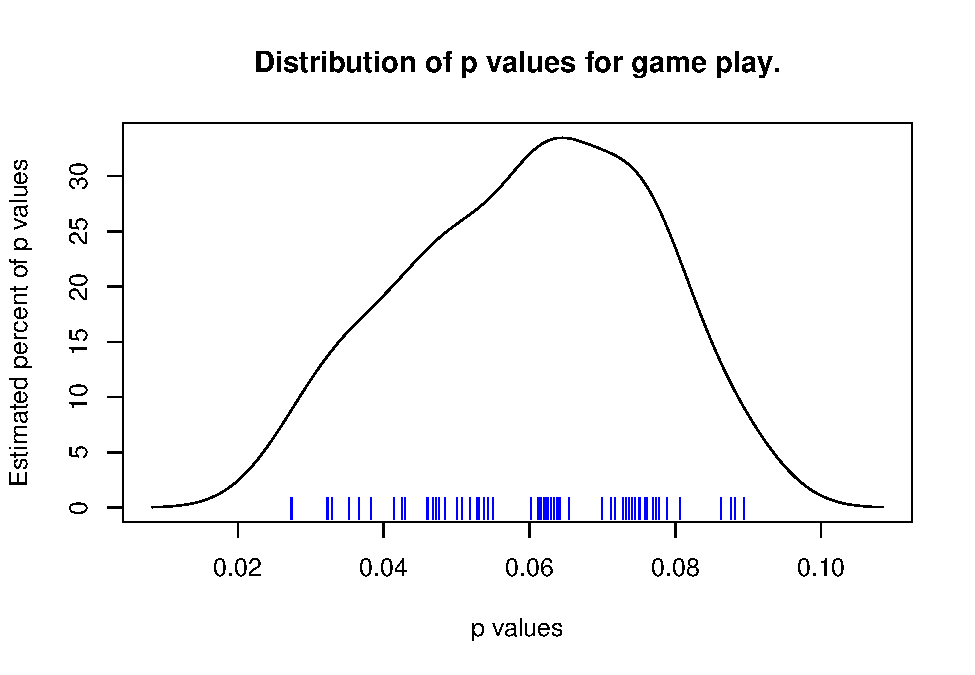
\includegraphics{stats_6_final_files/figure-latex/plotpfirst-1} 

}

\caption{Distribution of p values for different combinations of data for the linear component of the regression model of game play on the weekdays. Note that the curve does not represent the true probability distribution of the p values.}\label{fig:plotpfirst}
\end{figure}
\begin{figure}

{\centering 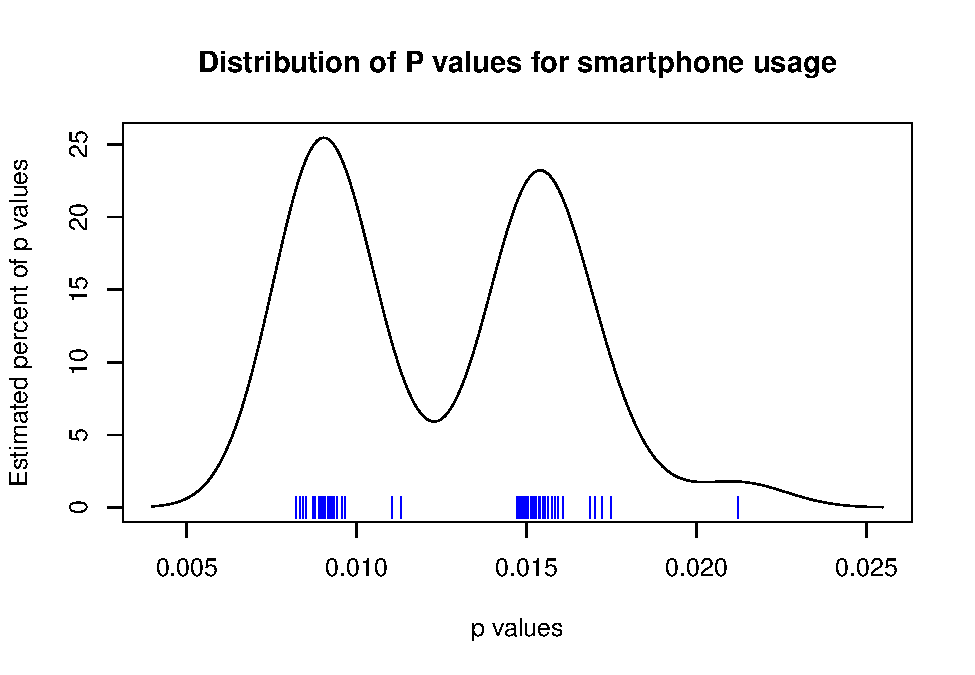
\includegraphics{stats_6_final_files/figure-latex/plotpsecond-1} 

}

\caption{Distribution of p values for different combinations of data for the linear component of the regression model of smartphone usage on weekdays. Note that the curve does not represent the true probability distribution of the p values.}\label{fig:plotpsecond}
\end{figure}

\begin{figure}
\centering
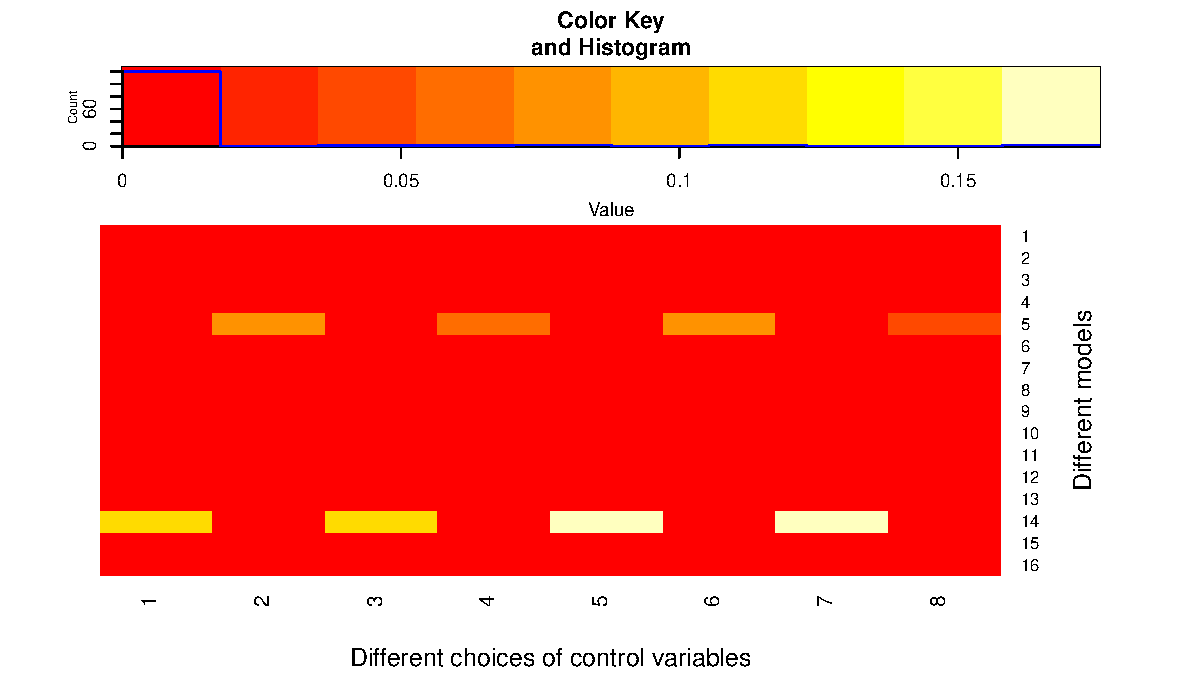
\includegraphics{stats_6_final_files/figure-latex/heat-p-model-1.pdf}
\caption{\label{fig:heat-p-model}Heat map of p values for different
decisions about inclusion/exclusion of control variables in the
regression models. Rows represents the coresponding rows in Table 1 and
2 and each column is for one of the 8 different inclusion/exclusion
combinations.}
\end{figure}

\begin{figure}
\centering
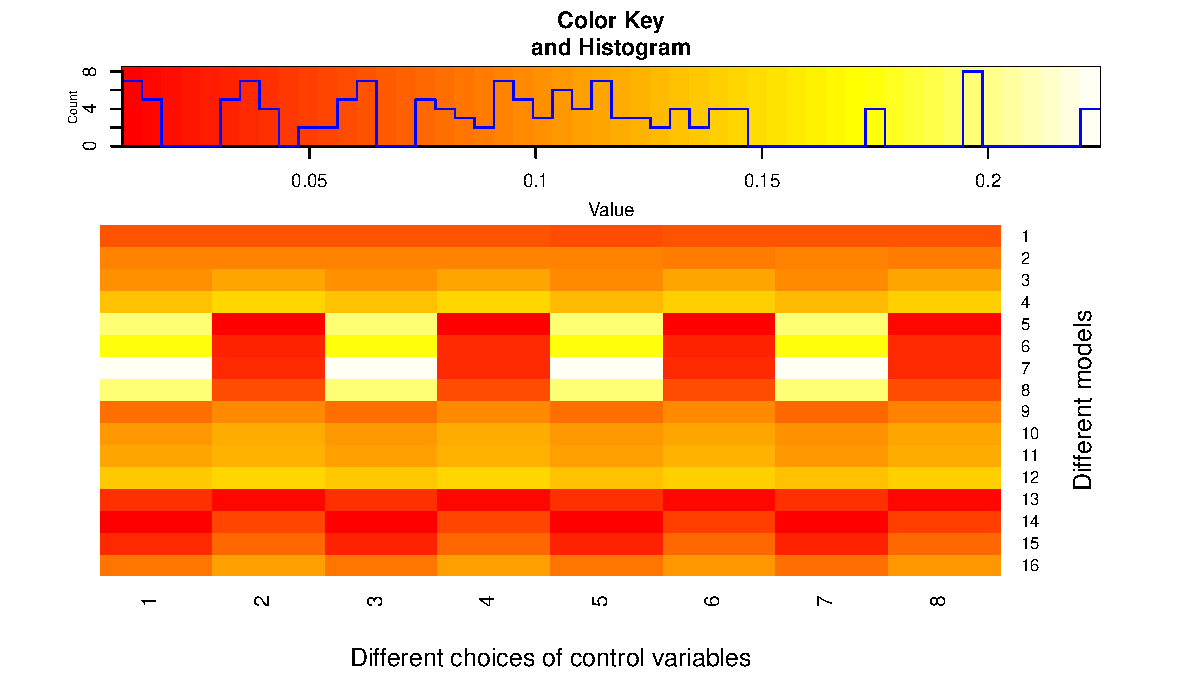
\includegraphics{stats_6_final_files/figure-latex/heat-d-model-1.pdf}
\caption{\label{fig:heat-d-model}Heat map of Cohen's d for different
decisions about inclusion/exclusion of control variables in the
regression models. Rows represents the coresponding rows in Table 1 and
2 and each column is for one of the 8 different inclusion/exclusion
combinations.}
\end{figure}

\begin{figure}
\centering
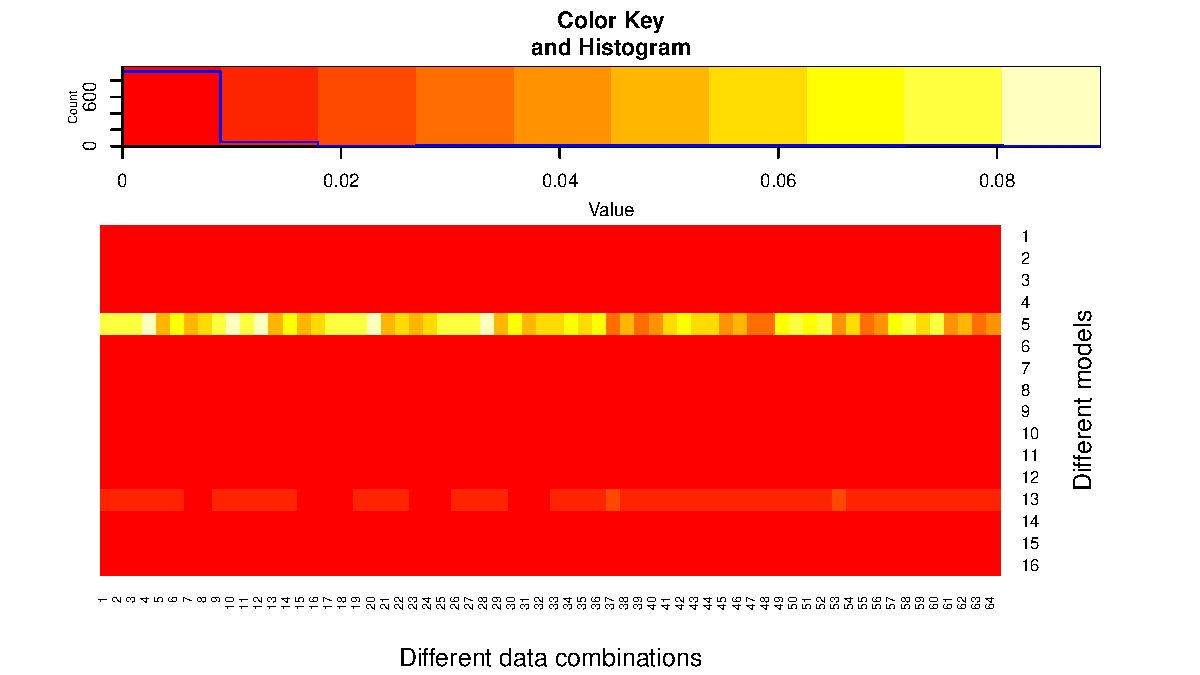
\includegraphics{stats_6_final_files/figure-latex/heat-p-data-1.pdf}
\caption{\label{fig:heat-p-data}Heat map of p values for different choices
of variable coding. Rows represents the coresponding rows in Table 1 and
2 and each column is for one of the 64 different data combinations.}
\end{figure}

\begin{figure}
\centering
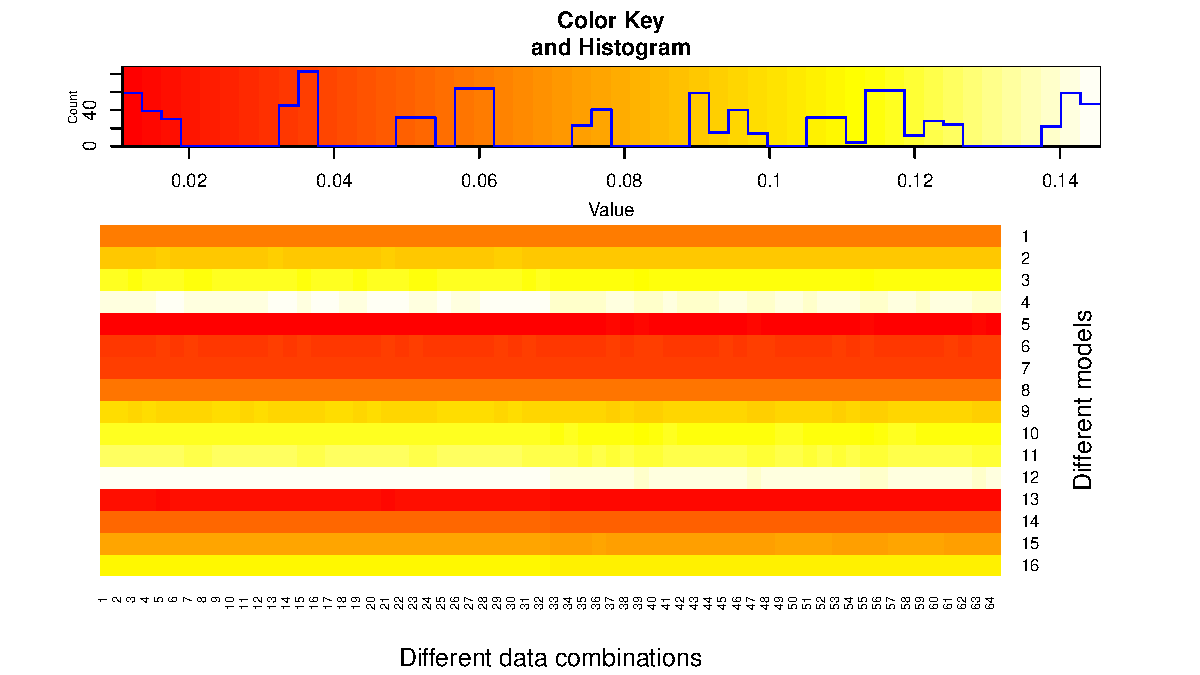
\includegraphics{stats_6_final_files/figure-latex/heat-d-data-1.pdf}
\caption{\label{fig:heat-d-data}Heat map of Cohen's d for different choices
of variable coding. Rows represents the corresponding rows in Table 1
and 2 and each column is for one of the 64 different data combinations.}
\end{figure}

Interestingly, we find that \emph{p} values corresponding to the linear
component of the regression model for weekday smartphone use is
significant (for a significance threshold of \(\alpha = 0.01\)) only for
\(0.47\%\) of the multiverse encapsulating all possible researcher
choices in variable coding. This percent drops to \(0\%\) for the linear
component of weekday game play. It is worth mentioning that for all
other models we do not observe any noticable change in the \emph{p}
values. Please note that the significance threshold was originally
suggested as \(\alpha = 0.001\) in the paper. However, since this
conservative threshold resulted in zero multiverse-frequencies, we
increased it to \(\alpha = 0.01\). These differences, along with the
difference in regression parameters reported above, can likely be
ascribed to the ambiguities mentioned throughout the paper.

\hypertarget{preregistration}{%
\subsubsection{Preregistration}\label{preregistration}}

The data were acquired according to the specifications made by the
authors in the preregistration document. However, in the technical
report on their OSF page, the authors said to use a 3\% margin of error
at the 95\%CI to estimate sample size. In the published paper, the
authors report a 0.3\% margin of error, arriving at the same estimate of
sample size (N = 298,080. Furthermore, The authors reported a total n of
120,115 participants with usable data. When we attempted to replicate
their analyses, we met with a further reduction of n to 98278. This is
not reported anywhere in the published article. Finally, the two data
documents provided by the authors differ in the amount of NA data they
contain. Where the .csv file contains 21837 rows with missing values,
the .sav file contains 44642 rows with missing values. None of these
inconsistencies were reported by the authors in the final paper, and it
is unclear which dataset the authors ultimately used in their analysis.
The fact that the data are ambiguous is a major obstacle for replication
analyses.

The preregistration document stated that testing the displacement
hypothesis was to be done by linear regression modeling, predicting
mental well-being through composite scores of screen time. The authors
did not conduct these analyses. They explain that \enquote{Interocular}
tests were sufficient to exclude this hypothesis. Although we only found
one unadjusted model for which the BIC criterium favors a purely linear
model, this does allow one to question why the authors refrained from
the formal hypothesis test detailed in the preregistration document.

The authors ignored the measure of summed screen time which they
included in their preregistration document. The authors reported this
accordingly, although our above analysis allows the questionability of
their deviation on this point. Finally, the authors did not concretely
specify what particular coding they intended to use for the control
variables of \enquote{whether living in a deprived area}, and
\enquote{whether black and minority ethnicity}. While the conditionality
of the term \enquote{whether} implies binary coding, the subsequent
reference to the specific questions would also allow one to assume that
the authors used the values from those questions. This is relevant
because other codings of these variables are also present in the data.
Although this is a minor issue, a more clear issue is also present. The
authors noted in their deviations from analysis plan that the
preregistered control variables of \enquote{whether parents married} and
\enquote{whether native-born}, they did not include the omission of
these variables in the published article.

\newpage

\hypertarget{references}{%
\section{References}\label{references}}

\begingroup
\setlength{\parindent}{-0.5in}
\setlength{\leftskip}{0.5in}

\hypertarget{refs}{}
\leavevmode\hypertarget{ref-przybylski2017large}{}%
Przybylski, A. K., \& Weinstein, N. (2017). A large-scale test of the
goldilocks hypothesis: Quantifying the relations between digital-screen
use and the mental well-being of adolescents. \emph{Psychological
Science}, \emph{28}(2), 204--215.

\leavevmode\hypertarget{ref-steegen2016increasing}{}%
Steegen, S., Tuerlinckx, F., Gelman, A., \& Vanpaemel, W. (2016).
Increasing transparency through a multiverse analysis.
\emph{Perspectives on Psychological Science}, \emph{11}(5), 702--712.

\endgroup






\end{document}
